
\subsection{Ikeda's method: from strip theory to semi-empirical formulas}
\label{se:semi-empirical methods}
Since the scale effect of the damping is mainly associated with the skin friction on ship hulls and the friction only contributes very little to a ship's total roll damping, the most reliable way to obtain a ship's roll damping coefficients is to carry out model scale experimental tests. 
While in a ship's early design stage when only limited information is available and flexible to be adjusted, such as the ship's principal dimensions and the basic hull geometry, some semi-empirical methods were also proposed to predict the roll damping \parencite{himeno_prediction_1981}. The most recognize method was developed in a series of research articles \parencite{ikeda_roll_1978,ikeda_eddy_1978,ikeda_roll_1979,ikeda_components_1978,ikeda_velocity_1979}, and it is well-known to be named as Ikeda's method. This method divides the roll damping into five damping components, i.e., the friction component $B_F$, the eddy component $B_e$, the lift component $B_L$, the wave component $B_W$ and the bilge keel component $B_BK$, as in the following Eq.(\ref{eq:ikeda}), 

\begin{equation} \label{eq:ikeda}
B = B_F + B_E + B_L + B_W + B_{BK}
\end{equation}

where the wave and eddy components require strip theory based hydrodynamic analysis to get the ship's shape coefficients. The hydrodynamic analysis requires to get a ship's exact hull geometries. All the roll damping components depends on ship speed and roll motion frequency. It might be time consumption to build the geometry model and perform the strip theory based hydrodynamic analysis. Sometimes, a ship's hull geometry is simply not available for such purposes. 

A \emph{Simplified Ikeda's method} was proposed by \parencite{kawahara_simple_2011} and is instead used in this study to calculate all the damping components including the eddy component $B_E$ and wave component $B_W$. The semi-empirical formulas describe the five roll damping components as functions of ship length $L_{pp}$, beam $B$, draft $T$  block coefficient $C_{b}$, motion frequency $\omega$, ship speed $V$, etc., for a given roll amplitude $\phi_a$ through,

\begin{equation} \label{eq:simplified_ikeda_equation}
\left( B_{44}, \  B_{F}, \  B_{W}, \  B_{E}, \  B_{BK}, \  B_{L}\right) = \operatorname{Ikeda_{simplified}}\left(L_{pp},beam,C_{b},A_{0},OG,\phi_{a},BK_{L},BK_{B},\omega,T,V\right)
\end{equation}


where $A_{0}$, $OG$, $BK_{L}$ and $BK_{B}$ represent a ship's wetted surface area, vertical distance from the origin to a ship's center of gravity, length and width of bilge keel, respectively. The detailed formulas within $f$ can be referred to \parencite{himeno_prediction_1981}.

%The Simplified Ikeda method \cite{kawahara_simple_2011} has been implemented \cite{alexandersson_martinlarsalbertrolldecay-estimators_2020} with the intention to be used both as a benchmark and maybe also as a sub-component of a new method. The examples from \cite{kawahara_simple_2011} was recalculated to check that the method has been implemented correctly. The authors have been unable to find other ways to validate the implementation, which introduces some uncertainty to the comparisons. The method has been implemented as a function where the total roll damping and its component is calcultated: 



The roll damping consists of linear and nonlinear components. At zero speed the nonlinear damping is caused by the two-dimensional separation at the bilge keel or near the bilge circle (Eddy damping $B_E$). While at speed the nonlinear damping is mainly caused by the hydrodynamic lift force on the hull, represented as lift damping $B_L$. $B_E$ vanishes at high speed ($F_n>0.15)$ \parencite{ikeda_components_1978}.
The wave damping also changes at speed. Ikeda \parencite{ikeda_components_1978} proposes a formula for the fraction between wave damping at speed and zero speed,

\begin{equation} \label{eq:wave_speed_correction}
\frac{B_W}{B_{W0}} = f(L, B, .....) 
\end{equation}



%\begin{figure}[h]
%    \centering
%    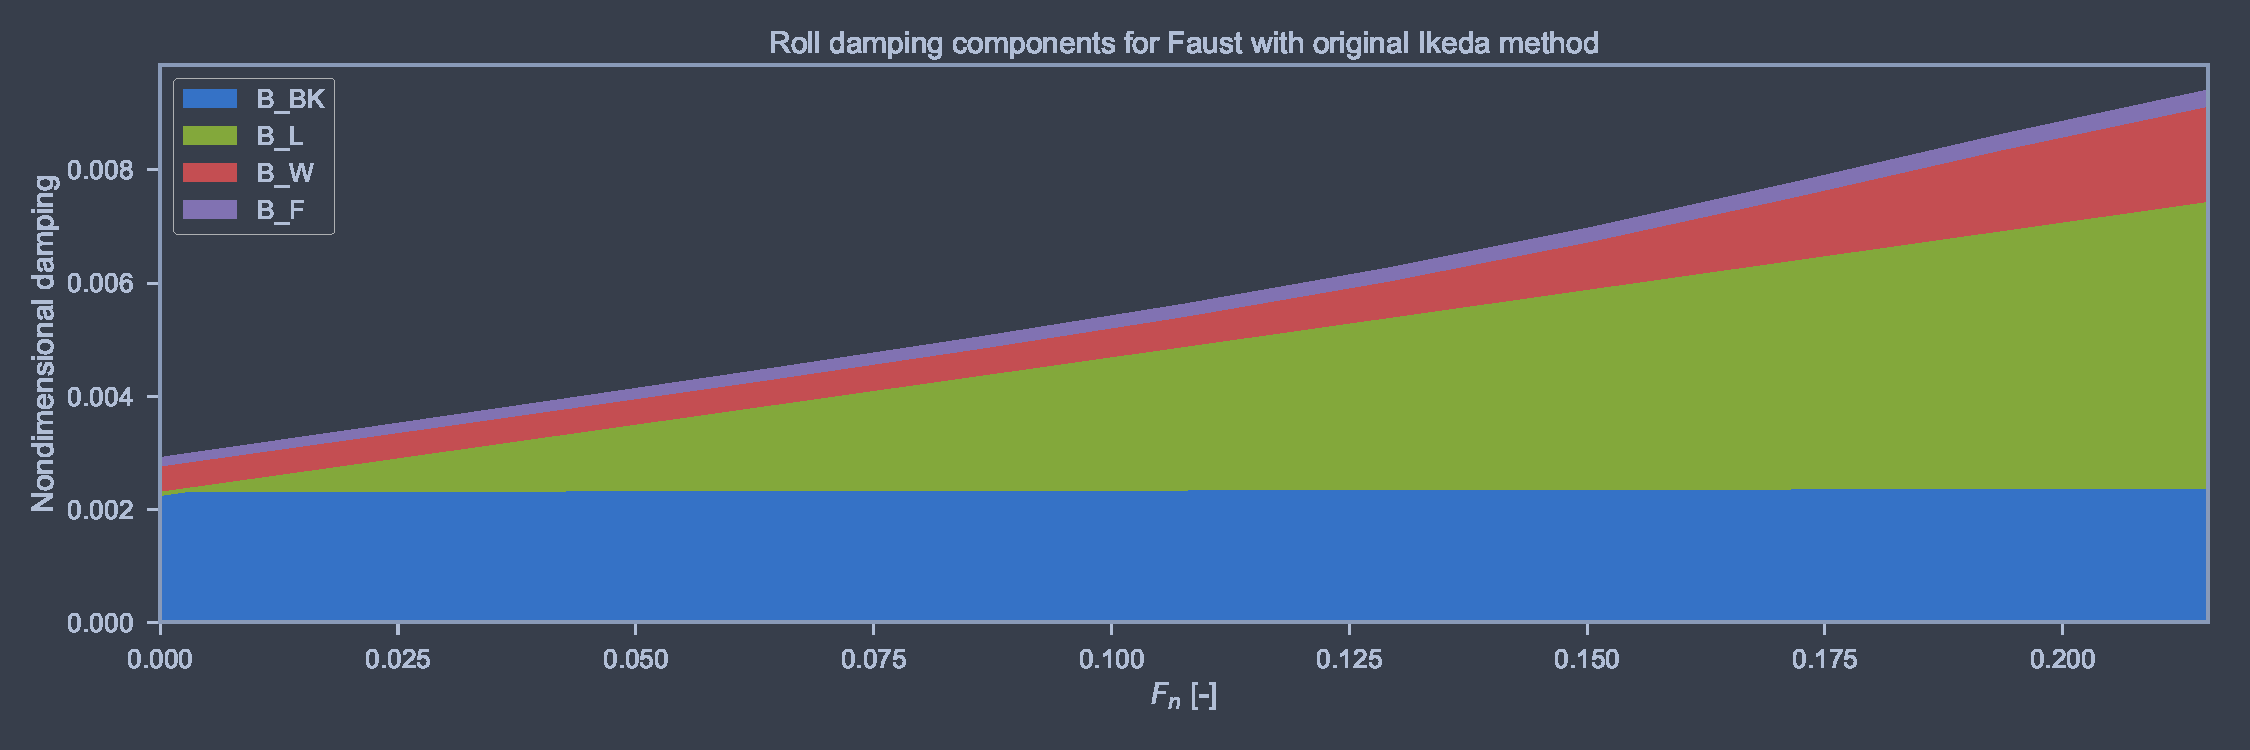
\includegraphics[width=\columnwidth]{figures/ikeda_faust.pdf}
%    \caption{Roll damping components calculated with Ikeda method for PCTC Faust}
%    \label{fig:ikeda_faust}
%\end{figure}





\begin{figure}[h]
    \centering
    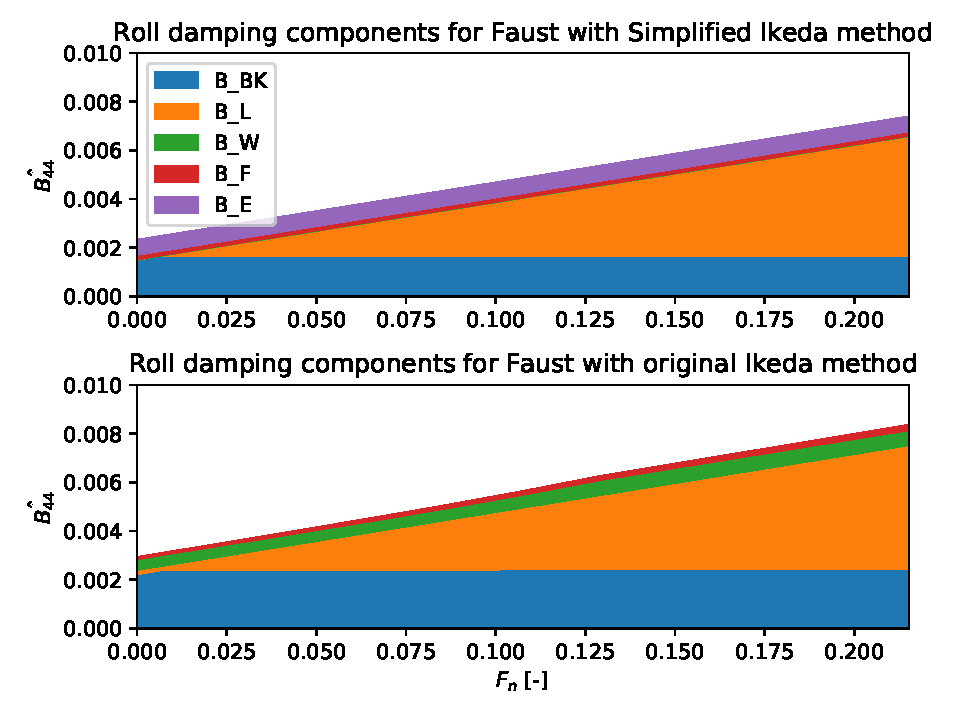
\includegraphics[height=7cm, width=14cm]{figures/ikeda_vs_simplified.pdf}
    \caption{Roll damping components calculated with Ikeda and Simplified Ikeda for PCTC Faust}
    \label{fig:ikeda_vs_simplified}
\end{figure}





A parameter variation was conducted in order to study the simplified method.
A "median ship" with the most usual parameters in the database was chosen as the baseline of the variation. The parameters were varied to the extreme values of the database, see figure \ref{fig:ship_parameters} for more details. 



The Ikeda method has been used to calculate the roll damping for a PCTC vessel Faust \parencite{soder_assessment_2019}. For example, Fig. \ref{fig:ikeda_vs_simplified} shows a comparison between roll damping components calculated with \emph{Ikeda} and \emph{Simplified Ikeda method}. The roll damping is under-predicted with the simplified method for this particular case which is expected according to the limitations of this method  \parencite{kawahara_simple_2011}.








Figure \ref{fig:ikeda_variation} shows this variation where all parameters have been none dimensionalized using froude scaling with $L_{pp}$ as scale factor. 
It seems that length to beam ratio between 0.23 and 0.24 has a huge peak. Also length to draft ratio below 0.034 has a large peak. 



\begin{figure}[H]
    \centering
    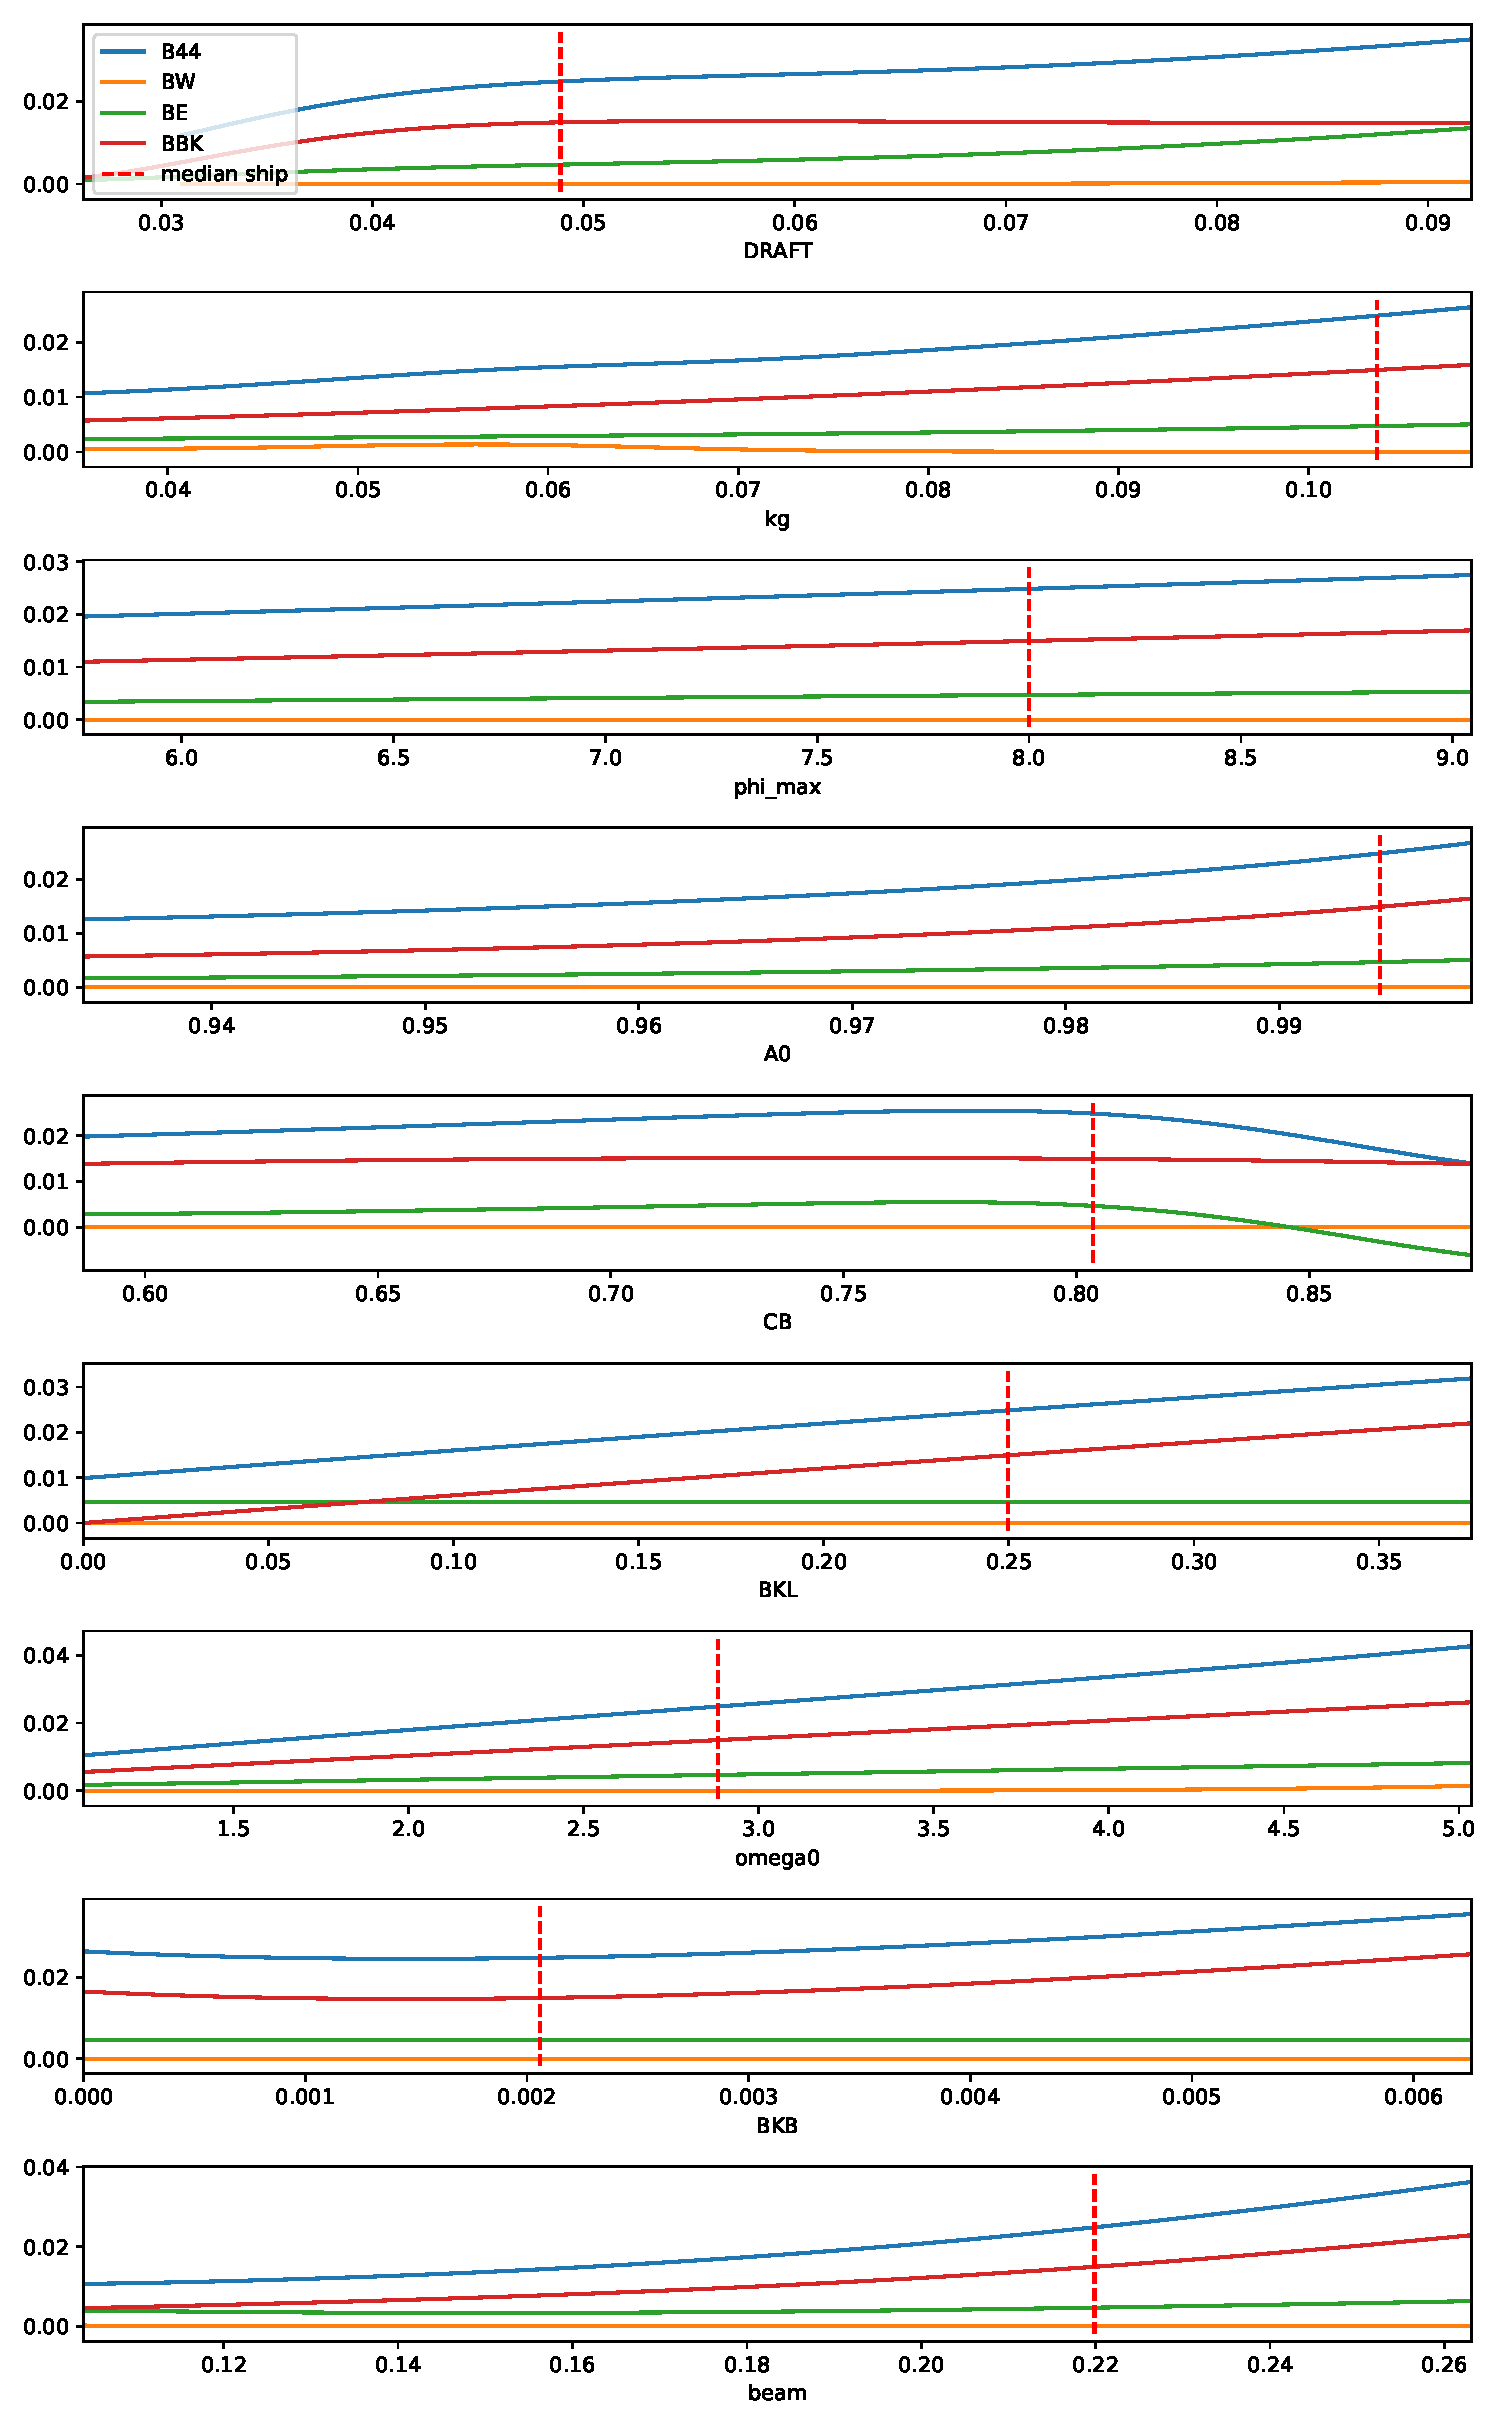
\includegraphics[height=13cm, width=15cm]{figures/ikeda_variation.pdf}
    \caption{Simplified method parameter variation}
    \label{fig:ikeda_variation}
\end{figure}

